\subsection{OSI参照モデル}

インターネットで利用されるプロトコルは、The Internet Engineering Task Force (IETF)という標準化
団体により策定され、その標準はRequest for Comments (RFC)という名のオープンな仕様として発行されている。
例えば、我々が利用しているインターネットプロトコルである
インターネットプロトコル バージョン4は、1981年に791番目のRFCとして策定された~\cite{RFC0791}。

IETF以外の通信に関する標準化団体としては
International Telecommunication Union Telecommunication Standardization Sector (ITU-T)や、
International Organization for Standardization (ISO)が存在する。
実は、1977年から1982年かけて、ITU-TやISOがコンピュータネットワークの標準通信プロトコルとして、
Open Systems Interconnection (OSI)の策定を行っていた。
その当時は標準的な通信プロトコルは存在せず、ベンダーごとに様々なプロトコルが利用されていたため、
通信プロトコルの統一化が求められていたのである。
しかしながら、最終的にOSIは主流とはならず、IETFによって策定された
インターネットプロトコルが広く利用されるようになっていった。

\begin{figure}[tb]
    \centering
    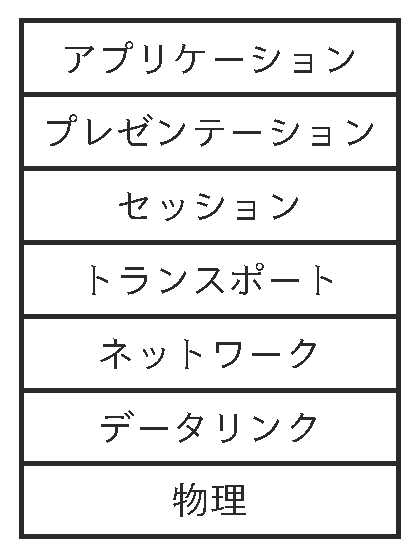
\includegraphics[width=5cm,pagebox=artbox]{figs/OSI.pdf}
    \caption{OSI参照モデル}
    \label{fig:osi}
\end{figure}

OSI自体は残らなかったが、OSI策定の際に考案されたOSI参照モデルと呼ばれる
ネットワークの抽象化手法は、今日でも広く受け入れられている。
図~\ref{fig:osi}は、OSI参照モデルによるネットワークの抽象化モデルを表している。
OSI参照モデルでは、ネットワークの機能を階層構造にもとづいて抽象化しており、
この抽象化をレイヤリングなどと呼ぶ。
OSI参照モデルでは、下から順に1層に物理層、2層にデータリンク層、
3層にネットワーク層、4層にトランスポート層、5層にセッション層、
6層にプレゼンテーション層、7層にアプリケーション層が位置する。
ちなみに、各層のことをレイヤ1、レイヤ2といったり、更に略してL1、L2などということもある。

\begin{figure}[tb]
    \centering
    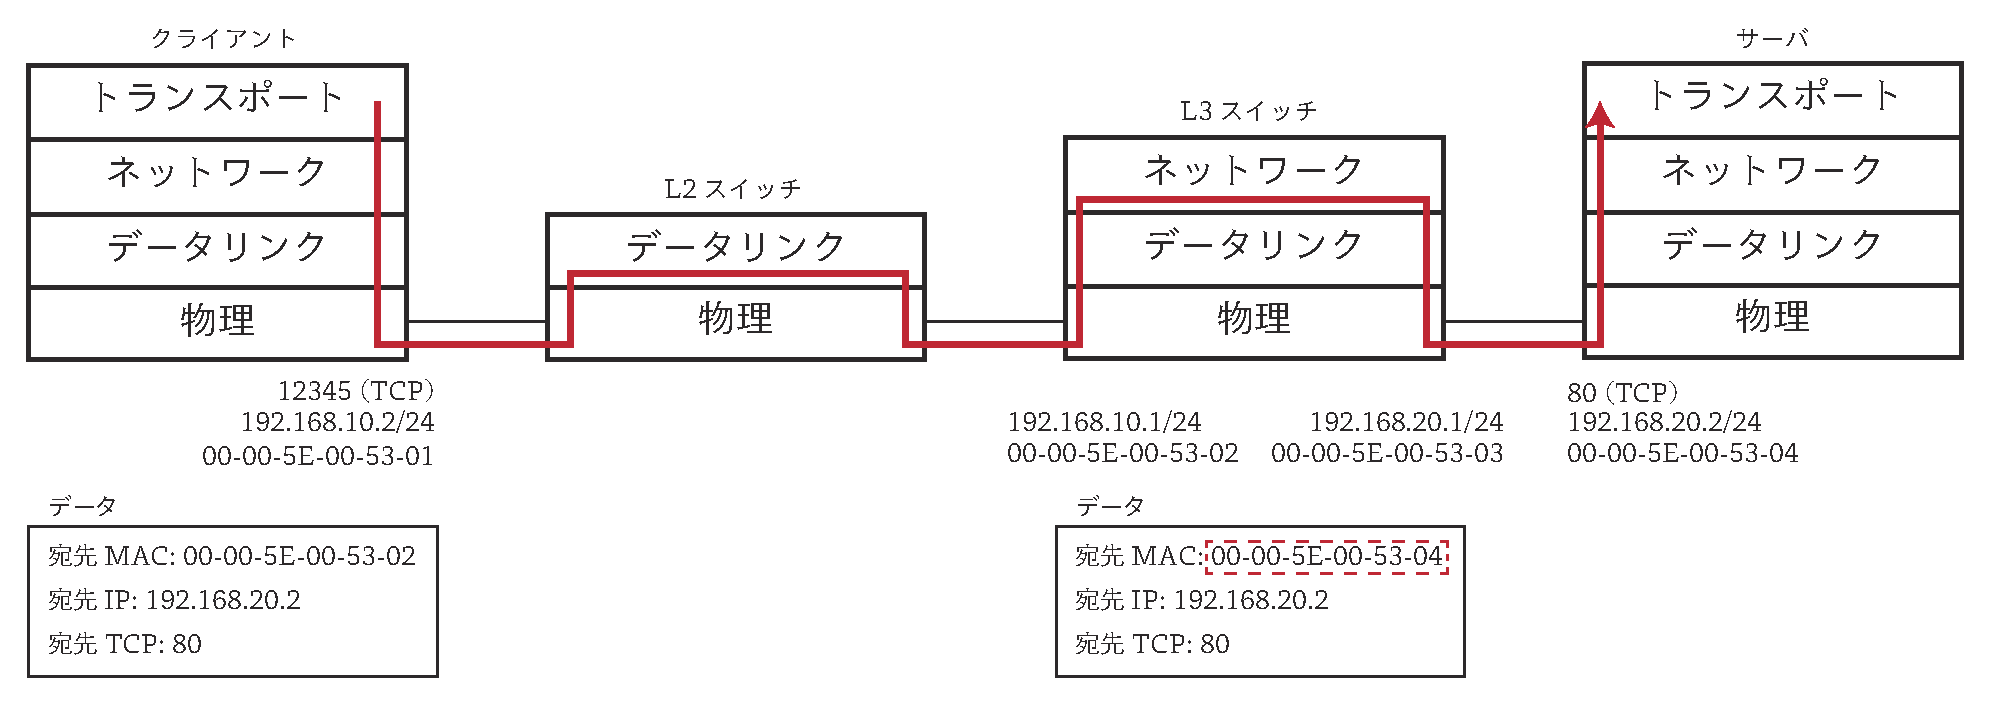
\includegraphics[width=14cm,pagebox=artbox]{figs/osi_link.pdf}
    \caption{各層でのデータ転送}
    \label{fig:osi_link}
\end{figure}

図~\ref{fig:osi_link}は各層でデータ転送が行われている様子を示している。
\footnote{
この図の意味することは現時点では理解できないかもしれないが、
この図の意味することろを説明するのが本節の目標であるため、
現段階で理解できなくても問題ない。
}
データリンク、ネットワーク、トランスポート層のプロトコルにはそれぞれアドレスがあり、
各層は、そのアドレスに基づいて転送を行う。
データリンク層プロトコルの一つであるIEEE 802では、アドレスは42ビットで表され、文字で表現すると00-00-5E-00-53-02といった
表記になる。
図~\ref{fig:osi_link}中で宛先MACと示される値は、
IEEE 802の宛先MACアドレスを示している。
なお、MACは Media Access Controlの略である。
データリンク層は、ローカルなネットワークでの通信を行うために用いられる。
そのため、MACアドレスはそのローカルな環境では一意に識別できる必要がある。
データリンク層の詳細については~\ref{sec:datalink}節で解説する。

ネットワーク層プロトコルの一つであるIPのアドレスは、192.168.10.2/24という32ビットの数値で表され、
/24はネットワークのサブネット長を示している。
図~\ref{fig:osi_link}では、192.168.10.0/24と192.168.20.0/24
というサブネットが示されている。
IPは、全世界で通信を行うために用いられるプロトコルであり、
基本的にはIPアドレスは世界で一意に識別できるように割り当てるのが設計理念となっている
(現実的にはそうはなっていないが)。
なお、前述のアドレスはIPv4アドレスであるが、IPv6の場合は128ビットのアドレス空間を持つ。
ネットワーク層の詳細については~\ref{sec:network}節で解説する。

トランスポート層プロトコルのTCPとUDPのアドレスは16ビットで示され、一般的にポート番号と呼ばれ、
TCPやUDPはポート番号をもとにアプリケーションプロセスの識別を行う。
よく利用されるポート番号は、インターネット上で利用される識別情報の管理割当を行っている
Internet Assigned Number Authority (IANA)が定義しており~\cite{wellknown}、
一般的にこのようなポート番号をWell Knownポート番号と呼ぶ。
例えば、TCPの80番ポートはHTTPで利用され、普段我々がWebを閲覧する際は、
WebブラウザがWebサーバのTCP80番ポートへ接続する。

図~\ref{fig:osi_link}では、クライントからサーバのTCP80番ポートへむけて
通信を行っている様子を示している。
一般的に、インターネット上の通信ではデータ中に含まれる各層のアドレスをもとに、
L2またはL3スイッチが転送を行う。
L2スイッチのことをスイッチングハブといったり、
L3スイッチのことをルータということもあるが、本書ではL2スイッチ、
L3スイッチと呼ぶことにする。
この図が示すように、L2スイッチ、L3スイッチによってデータが転送されても、
データ中のIPアドレスとポート番号は変わらないが、MACアドレスはL3スイッチでの転送時に更新される。
これは、MACアドレスはローカルなネットワーク内でのみ通用するアドレスであり、
L3スイッチはローカルなネットワーク同士をつなぎ合わせる役割を持っているためである。
以降の節では、データリンク、ネットワーク、トランスポートの動きについて詳しく説明する。

\begin{itembox}[l]{\bf 重要ポイント}
    \begin{itemize}
        \item インターネット関連のプロトコルは、IETFが発行するRFCによって標準化されている
        \item コンピュータネットワークはレイヤで考えることができる
        \item Ethernetのアドレスは48ビットのMACアドレス、IPv4のアドレスは32ビットのIPv4アドレス、IPv6のアドレスは128ビットのIPv6アドレス、TCPとUDPのアドレスは16ビットのポート番号
    \end{itemize}
\end{itembox}

\subsection{おもちゃのネットワークスタック} \label{sec:stack}

\begin{figure}[tb]
    \centering
    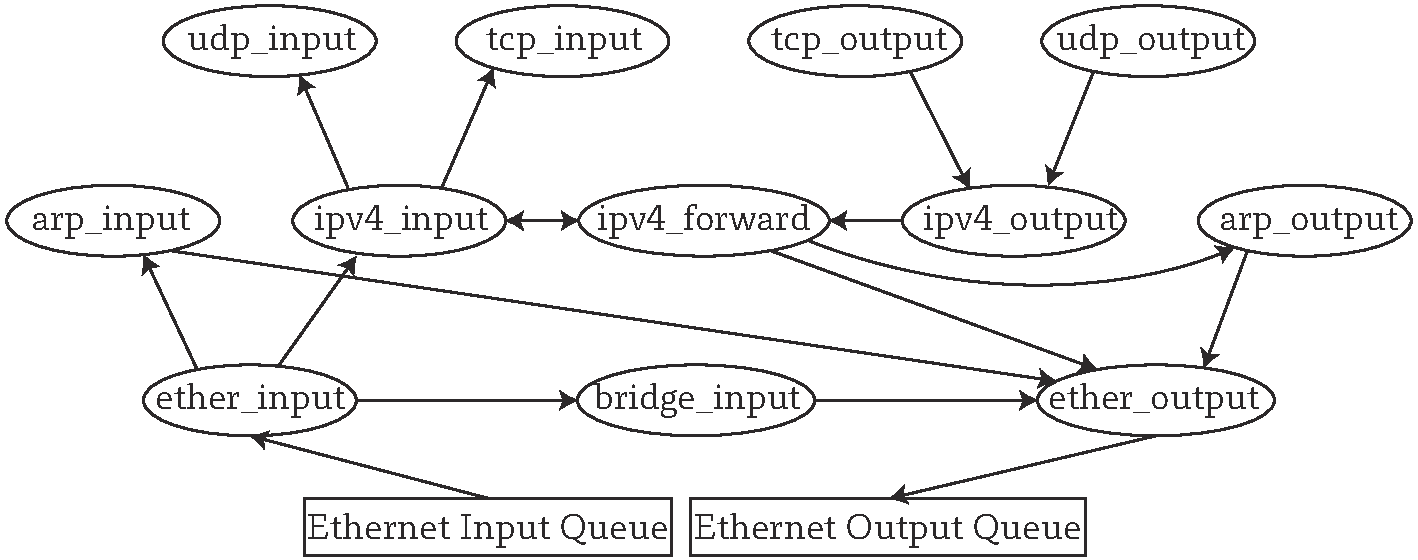
\includegraphics[width=14cm,pagebox=artbox]{figs/nwstack.pdf}
    \caption{おもちゃのネットワークスタックのデータフロー図}
    \label{fig:tcpipstack}
\end{figure}

これより本章では、おもちゃのネットワークスタックを用いて、
ネットワークスタックの設計と実装を解説する。
おもちゃと言っても、実際にIPルータやEthernetブリッジとして動作するれっきとしたネットワークスタックである。
図~\ref{fig:tcpipstack}はおもちゃのネットワークスタックのデータフロー図を示している。
この図の下部には、入力と出力用のEthernet Input/Ouptput Queueというキューがあり、
ここで物理的な入出力が行われる。
実際に、ネットワークインターフェースカードには入出力用のキューが用意されており、
デバイスドライバはこれらキューに対して読み書きすることでデータの送受信を行う。

なお、このおもちゃのネットワークは、Ethernetブリッジや、IPv4のルーティングは行うことができるが、
TCPのセッション管理などは行えないし、扱えるのは基本的にユニキャストのみで、マルチキャスト通信はサポートしていない。
また、実際のOSではネットワークスタックの上にソケットレイヤが配置され、
ネットワークに関する操作が抽象化されているが、おもちゃのネットワークスタックではソケットレイヤは省略されている。
すなわち、あくまでも、ファイアウォールなどを理解して運用するために必要最低限と思われる機能のみが実装されている。

\subsection{ネットワークインターフェース} \label{sec:nwif}

スタックの説明を行う前に、ネットワークインターフェース情報を表すための構造体を説明しよう。
ソースコード~\ref{src:my_ifnet.h}は、おもちゃのネットワークスタックで定義するネットワークインターフェース用のmy\_ifnet構造体となる。

\begin{lstlisting}[caption=ネットワークインターフェースを表す構造体 (my\_ifnet.h),label=src:my_ifnet.h]
// インターフェース情報を保持する構造体
struct my_ifnet {
    int idx;                       // インデックス
    uint8_t ifaddr[6];             // MACアドレス
    struct in_addr addr;           // IPv4アドレス
    struct in6_addr addr6;         // IPv6アドレス
    uint8_t plen;                  // IPv4プレフィックス長
    uint8_t plen6;                 // IPv6プレフィックス長
    char infile[128];              // 入力UNIXファイル名
    char outfile[128];             // 出力UNIXファイル名
    int sockfd;                    // 入力先UNIXドメインソケット
    struct sockaddr_un outun;      // 出力UNIXアドレス
    LIST_ENTRY(my_ifnet) pointers; // リスト
};
\end{lstlisting}

my\_ifnet構造体のメンバ変数は基本的にはコメントにあるとおりだが、もう少し詳しく説明したのが
表~\ref{tab:my_ifnet}となる。
表~\ref{tab:my_ifnet}で示すように、ネットワークインターフェースには各種アドレスが紐付けられる。
また、おもちゃのネットワークスタックでは、データの送受信にUNIXドメインソケットのデータグラム通信を行うため、
UNIXドメインソケット用のデータがいくつが用意されている。

\begin{table}[tb]
    \centering
    \caption{my\_ifnet構造体のメンバ変数} \label{tab:my_ifnet}
    \begin{tabular}{rl}
        idx & 複数インターフェースの番号を識別するためのメンバ変数 \\
        addr & インターフェースに対応付けられたIPv4アドレス \\
        addr6 & インターフェースに対応付けられたIPv6アドレス \\
        plen & IPv4プレフィックスアドレス(\ref{sec:network}節にて解説) \\
        plen6 & IPv6プレフィックスアドレス(\ref{sec:network}節にて解説) \\
        infile & データ受信を行うためのUNIXドメインソケットへのファイル名 \\
        outfile & データ送信を行うためのUNIXドメインソケットへのファイル名 \\
        sockfd & データ受信用のUNIXドメインソケットへのデスクリプタ \\
        outun & データ送信用のUNIXドメインソケットへのアドレス \\
        pointers & 複数インターフェースをリストで管理するためのポインタ。sys/queue.hを利用 \\
    \end{tabular}
\end{table}

ソースコード~\ref{tab:my_ifnet}はおもちゃのネットワークスタックの割り込みハンドラを表している。
割り込みハンドラとは、ネットワークカードにデータが到着した際に呼び出される関数のことを指す。
実際のOSでは物理的な入力が割り込みハンドラを起動するが、おもちゃのネットワークスタックでは
UNIXドメインソケットへの入力があったときにdev\_input関数を呼び出すようにしている。

\begin{lstlisting}[caption=割り込みハンドラ (my\_ifnet.c),label=src:my_ifnet.c]
/*
 * インターフェース入力割り込み関数
 * 引数:
 *   fd: UNIXドメインソケットへのファイルデスクリプタ
 */
void dev_input(int fd) {
    for (struct my_ifnet *np = LIST_FIRST(&ifs); np != NULL;
         np = LIST_NEXT(np, pointers)) {
        if (np->sockfd == fd) {
            char buf[4096];
            ssize_t size;
        again:
            size = recv(fd, buf, sizeof(buf), 0);
            if (size < 0) {
                if ((errno) == EAGAIN)
                    goto again;

                perror("recv");
                break;
            }

            ether_input(np, (struct ether_header *)buf, size);
            break;
        }
    }
}
\end{lstlisting}

ソースコード~\ref{tab:my_ifnet}では引数に入力用のUNIXドメインソケットを受け取り、
7〜8行目で対応するUNIXドメインソケットを持つmy\_ifnet構造体をリストから検索している。
入力インターフェースのmy\_ifnet構造体が見つかったら(9行目)、13行目でデータ読み込みを行っている。
14〜20行目エラー処理で、読み込みに失敗した場合はerrnoがEAGAINであれば、再度読み直し
それ以外であれば読み込み失敗として関数を抜ける。
データを読み込んだ後、22行目でether\_input関数を呼び出して実際の処理に入る。
これは図~\ref{fig:tcpipstack}で示される、Ethernet Input Queueからether\_input関数へのデータフローに相当する。

\begin{itembox}[l]{\bf 重要ポイント}
    \begin{itemize}
        \item ネットワークインターフェースカードにデータが到着した際に、OSで設定した割り込みハンドラと呼ばれる関数が呼び出される
        \item 割り込みハンドラから、実際にネットワーク処理を行うための関数が呼ばれる
    \end{itemize}
\end{itembox}

\subsection{データリンク層} \label{sec:datalink}

ソースコード~\ref{src:if_ether.h}はEthernet (IEEE 802.3) プロトコルのヘッダ構造体を示している。
我々が普段利用している無線や有線のEthernetでは、内部的にはこのようなフォーマットのヘッダがデータの先頭に付与され、
その後にIPヘッダ、TCPヘッダなどのより上位のヘッダが続き、最後にアプリケーションデータが続く。
もう少し正確に言うと、ソースコード~\ref{src:if_ether.h}で示すEthernetヘッダの前にプリアンブルなどの
ハードウェアで利用されるデータが続くが、本書ではその説明は割愛する。

\begin{lstlisting}[caption=Ethernetプロトコルヘッダ定義 (/usr/include/netinet/if\_ether.h),label=src:if_ether.h]
#define ETHER_ADDR_LEN  6       /* Ethernet address length              */

/*
 * The length of the combined header.
 */
struct  ether_header {
        u_int8_t  ether_dhost[ETHER_ADDR_LEN];
        u_int8_t  ether_shost[ETHER_ADDR_LEN];
        u_int16_t ether_type;
};
\end{lstlisting}

ソースコード~\ref{src:if_ether.h}で示されるように、
Ethernetヘッダの構造体は、OpenBSDでは、/usr/include/netinet/if\_ether.h にて定義されている。
なお、以降特に断りがない限り対象とするOSはOpenBSDとし、/usr/includeのパスから始まるソースコードは、
OSが提供するソースコードであるとする。
1行目のETHER\_ADDR\_LENでは、Ethernetアドレス(MACアドレス)のバイト数を6バイトと定義している。
6行目以降がEthernetヘッダを示すether\_header構造体となる。
ether\_header構造体では、ether\_dhostとether\_shostというメンバ変数を持ち、
それぞれ宛先MACアドレスと送信元MACアドレスを示している。
ether\_typeメンバ変数は、Ethernetヘッダ以降に続くプロトコル種類を示している。

ether\_typeメンバ変数で利用できる値はIANAによって定義されている~\footnote{\url{https://www.iana.org/assignments/ieee-802-numbers/ieee-802-numbers.xhtml} (ethernet type ianaで検索)}。
例えば、IPv4が続く場合は16進数表記で0x0800という値がether\_typeに格納される。
他には、IPv6の場合は0x08DD、仮想的なLANを構築するためのIEEE 802.1Q VLANプロトコルの場合は0x8100が格納される。

\begin{lstlisting}[caption=ether\_input関数 (ether.c),label=src:ether_input]
/*
 * Ethernetフレーム入力関数
 * 引数:
 *   ifp: 入力インターフェース
 *   eh: 入力フレーム
 *   len: 入力フレーム長
 */
void ether_input(struct my_ifnet *ifp, struct ether_header *eh, int len) {
    printf("ether_input:\n");
    printf("    IF#: %d\n", ifp->idx);
    printf("    SRC MAC: %02X-%02X-%02X-%02X-%02X-%02X\n", eh->ether_shost[0],
           eh->ether_shost[1], eh->ether_shost[2], eh->ether_shost[3],
           eh->ether_shost[4], eh->ether_shost[5]);
    printf("    DST MAC: %02X-%02X-%02X-%02X-%02X-%02X\n", eh->ether_dhost[0],
           eh->ether_dhost[1], eh->ether_dhost[2], eh->ether_dhost[3],
           eh->ether_dhost[4], eh->ether_dhost[5]);
    printf("\n");

    if (IS_BROADCAST(eh->ether_dhost)) {
        // ブロードキャストアドレスの場合、ブリッジ処理へ
        if (IS_L2BRIDGE)
            bridge_input(ifp, eh, len);
    } else if (memcmp(ifp->ifaddr, eh->ether_dhost, ETHER_ADDR_LEN) != 0) {
        // 宛先MACアドレスが自インターフェース宛でないならブリッジ処理を行い終了
        if (IS_L2BRIDGE)
            bridge_input(ifp, eh, len);
        return;
    }

    switch (ntohs(eh->ether_type)) {
    case ETHERTYPE_IP: // IPv4入力
        ipv4_input((struct ip *)((uint8_t *)eh + ETHER_HDR_LEN));
        break;
    case ETHERTYPE_IPV6: // IPv6入力
        ipv6_input((struct ip6_hdr *)((uint8_t *)eh + ETHER_HDR_LEN));
        break;
    case ETHERTYPE_ARP: // ARP入力
        arp_input(ifp, (struct arphdr *)((uint8_t *)eh + ETHER_HDR_LEN));
        break;
    default:
        printf("eh->ether_type is neither IPv6 nor IPv6\n");
        return;
    }

    return;
}\end{lstlisting}

ソースコード~\ref{src:ether_input}はおもちゃのネットワークスタックのEthernetフレームを受け取り処理を行うethernet\_input関数である。

\subsection{ネットワーク層} \label{sec:network}

\begin{lstlisting}[caption=IPv4ヘッダ定義 (/usr/include/netinet/ip.h),label=src:ip.h]
/*
 * Structure of an internet header, naked of options.
 */
struct ip {
#if _BYTE_ORDER == _LITTLE_ENDIAN
        u_int     ip_hl:4,              /* header length */
                  ip_v:4;               /* version */
#endif
#if _BYTE_ORDER == _BIG_ENDIAN
        u_int     ip_v:4,               /* version */
                  ip_hl:4;              /* header length */
#endif
        u_int8_t  ip_tos;               /* type of service */
        u_int16_t ip_len;               /* total length */
        u_int16_t ip_id;                /* identification */
        u_int16_t ip_off;               /* fragment offset field */
#define IP_RF 0x8000                    /* reserved fragment flag */
#define IP_DF 0x4000                    /* dont fragment flag */
#define IP_MF 0x2000                    /* more fragments flag */
#define IP_OFFMASK 0x1fff               /* mask for fragmenting bits */
        u_int8_t  ip_ttl;               /* time to live */
        u_int8_t  ip_p;                 /* protocol */
        u_int16_t ip_sum;               /* checksum */
        struct    in_addr ip_src, ip_dst; /* source and dest address */
};
\end{lstlisting}

\begin{lstlisting}[caption=IPv6アドレス構造体 (/usr/include/netinet6/in6.h),label=src:in6.h]
/*
 * IPv6 address
 */
struct in6_addr {
        union {
                u_int8_t   __u6_addr8[16];
                u_int16_t  __u6_addr16[8];
                u_int32_t  __u6_addr32[4];
        } __u6_addr;                    /* 128-bit IP6 address */
};
\end{lstlisting}

\begin{lstlisting}[caption=IPv6ヘッダ定義 (/usr/include/netinet/ip6.h),label=src:ip6.h]
/*
 * Definition for internet protocol version 6.
 * RFC 2460
 */

struct ip6_hdr {
        union {
                struct ip6_hdrctl {
                        u_int32_t ip6_un1_flow; /* 20 bits of flow-ID */
                        u_int16_t ip6_un1_plen; /* payload length */
                        u_int8_t  ip6_un1_nxt;  /* next header */
                        u_int8_t  ip6_un1_hlim; /* hop limit */
                } ip6_un1;
                u_int8_t ip6_un2_vfc;   /* 4 bits version, top 4 bits class */
        } ip6_ctlun;
        struct in6_addr ip6_src;        /* source address */
        struct in6_addr ip6_dst;        /* destination address */
} __packed;
\end{lstlisting}

\subsection{トランスポート層} \label{sec:transport}

\begin{lstlisting}[caption=TCPヘッダ定義 (/usr/include/netinet/tcp.h),label=src:tcp.h]
typedef u_int32_t tcp_seq;

/*
 * TCP header.
 * Per RFC 793, September, 1981.
 */
struct tcphdr {
        u_int16_t th_sport;             /* source port */
        u_int16_t th_dport;             /* destination port */
        tcp_seq   th_seq;               /* sequence number */
        tcp_seq   th_ack;               /* acknowledgement number */
#if _BYTE_ORDER == _LITTLE_ENDIAN
        u_int32_t th_x2:4,              /* (unused) */
                  th_off:4;             /* data offset */
#endif
#if _BYTE_ORDER == _BIG_ENDIAN
        u_int32_t th_off:4,             /* data offset */
                  th_x2:4;              /* (unused) */
#endif
        u_int8_t  th_flags;
#define TH_FIN    0x01
#define TH_SYN    0x02
#define TH_RST    0x04
#define TH_PUSH   0x08
#define TH_ACK    0x10
#define TH_URG    0x20
#define TH_ECE    0x40
#define TH_CWR    0x80
        u_int16_t th_win;                       /* window */
        u_int16_t th_sum;                       /* checksum */
        u_int16_t th_urp;                       /* urgent pointer */
};
\end{lstlisting}

\begin{lstlisting}[caption=UDPヘッダ定義 (/usr/include/netinet/udp.h),label=src:udp.h]
/*
 * Udp protocol header.
 * Per RFC 768, September, 1981.
 */
struct udphdr {
        u_int16_t uh_sport;             /* source port */
        u_int16_t uh_dport;             /* destination port */
        u_int16_t uh_ulen;              /* udp length */
        u_int16_t uh_sum;               /* udp checksum */
};
\end{lstlisting}

\subsection{トランスポートより上の層}